% VLDB template version of 2020-08-03 enhances the ACM template, version 1.7.0:
% https://www.acm.org/publications/proceedings-template
% The ACM Latex guide provides further information about the ACM template

\documentclass[sigconf, nonacm]{acmart}
\usepackage[utf8]{inputenc}
\usepackage[ruled,vlined]{algorithm2e}
\usepackage{amsmath}
\usepackage{listings}
\usepackage{tikz}
\usepackage{xcolor} % 包含颜色功能
\usepackage{amsthm}
\usepackage{subcaption}
\usepackage{booktabs}
\usepackage{threeparttable}
\usepackage{enumitem}
\renewcommand{\arraystretch}{1.4} % Increase row height for better spacing

% Add these lines after documentclass
\sloppy
\raggedbottom

%% The following content must be adapted for the final version
% paper-specific
\newcommand\vldbdoi{XX.XX/XXX.XX}
\newcommand\vldbpages{XXX-XXX}
% issue-specific
\newcommand\vldbvolume{14}
\newcommand\vldbissue{1}
\newcommand\vldbyear{2020}
% should be fine as it is
\newcommand\vldbauthors{\authors}
\newcommand\vldbtitle{\shorttitle} 
% leave empty if no availability url should be set
\newcommand\vldbavailabilityurl{URL_TO_YOUR_ARTIFACTS}
% whether page numbers should be shown or not, use 'plain' for review versions, 'empty' for camera ready
\newcommand\vldbpagestyle{plain} 

\begin{document}
\title{Helios: A Lightweight Path-driven Execution Engine for Hyper-Optimized EVM Clients}

%%
%% The "author" command and its associated commands are used to define the authors and their affiliations.
\author{Sipeng Xie$^\text{1}$, Qianhong Wu$^\text{1}$, Wenkuan Xiao$^\text{1}$, Mingzhe Zhai$^\text{1}$, Kun Wang$^\text{1}$, Qiyuan Gao$^\text{1}$, and Bo Qin$^\text{2}$}

\affiliation{%
    $^\text{1}$Beihang University, Beijing, China \quad
    $^\text{2}$Renmin University of China, Beijing, China
}
\affiliation{\{sipengxie, qianhong.wu, wenkuanxiao, zhaimingzhe, kun\_wang, gaoqy\}@buaa.edu.cn}
\email{bo.qin@ruc.edu.cn}

%%
%% The abstract is a short summary of the work to be presented in the
%% article.
% \input{chapters/00-abstract}
\begin{abstract}
    this is abstract.
\end{abstract}

\maketitle

%%% do not modify the following VLDB block %%
%%% VLDB block start %%%
\pagestyle{\vldbpagestyle}
\begingroup\small\noindent\raggedright\textbf{PVLDB Reference Format:}\\
\vldbauthors. \vldbtitle. PVLDB, \vldbvolume(\vldbissue): \vldbpages, \vldbyear.\\
\href{https://doi.org/\vldbdoi}{doi:\vldbdoi}
\endgroup
\begingroup
\renewcommand\thefootnote{}\footnote{\noindent
This work is licensed under the Creative Commons BY-NC-ND 4.0 International License. Visit \url{https://creativecommons.org/licenses/by-nc-nd/4.0/} to view a copy of this license. For any use beyond those covered by this license, obtain permission by emailing \href{mailto:info@vldb.org}{info@vldb.org}. Copyright is held by the owner/author(s). Publication rights licensed to the VLDB Endowment. \\
\raggedright Proceedings of the VLDB Endowment, Vol. \vldbvolume, No. \vldbissue\ %
ISSN 2150-8097. \\
\href{https://doi.org/\vldbdoi}{doi:\vldbdoi} \\
}\addtocounter{footnote}{-1}\endgroup
%%% VLDB block end %%%

%%% do not modify the following VLDB block %%
%%% VLDB block start %%%
\ifdefempty{\vldbavailabilityurl}{}{
\vspace{.3cm}
\begingroup\small\noindent\raggedright\textbf{PVLDB Artifact Availability:}\\
The source code, data, and/or other artifacts have been made available at \url{\vldbavailabilityurl}.
\endgroup
}

%%% VLDB block end %%%
\section{Introduction}

Public blockchains supporting smart contracts, such as Ethereum and its Layer-2 rollups~\cite{ethereum,base,arbitrum,polygon,bsc}, fundamentally operate as replicated state machines. From a data management perspective, each node functions as a deterministic transaction processor handling two distinct workloads. These workloads comprise the real-time processing of incoming transactions and the re-execution of historical transactions to verify global state transitions. As throughput and contract complexity increase, execution becomes a primary scalability bottleneck for both scenarios.

Recent acceleration strategies face distinct limitations on modern execution engines~\cite{revm,evmone}. Just-In-Time (JIT) compilation introduces security risks, such as JIT bombs, and causes gas accounting discrepancies~\cite{revmc,monad,evmjit,bnbjit,JITBomb}. Transaction-level speculative execution degrades performance on fast engines due to the \textit{Performance Paradox}~\cite{forerunner,seer}. In this phenomenon, the overhead of instrumentation, tracing, and artifact management frequently exceeds the latency of transaction execution itself. Similarly, operation-level concurrent execution incurs tracing or synchronization costs that frequently outweigh parallel gains~\cite{parallelEvm,evmTracer}.

Overcoming the performance paradox on hyper-optimized EVM clients necessitates addressing three fundamental conflicts. \textbf{First}, the tension between instrumentation overhead and execution latency. On sub-microsecond engines such as Revm~\cite{revm}, the cost of synchronous tracing often exceeds the execution time itself. Capturing sufficient data dependencies without introducing latency that negates the speedup is non-trivial. \textbf{Second}, the trade-off between artifact granularity and reuse capability. Existing transaction-level approaches suffer from a combinatorial explosion of unique execution paths, rendering cached artifacts ephemeral. The challenge lies in identifying a stable granularity that exhibits high locality across diverse transactions while maintaining manageable storage costs. \textbf{Third}, the conflict between optimization aggressiveness and strict semantic preservation. Standard compiler transformations such as instruction reordering inherently alter observable execution steps and violate the EVM's gas accounting rules. Achieving significant opcode reduction without complex runtime compensation logic remains a critical hurdle.

To assess whether these challenges can be surmounted, we analyzed Ethereum mainnet workloads and derived three critical insights. \textbf{First}, on hyper-optimized clients, native memory and storage management is already highly efficient; capturing full execution state incurs prohibitive I/O overhead while offering negligible optimization utility. Critical dependencies for valid optimization are therefore sparse and confined to stack operations, making lightweight stack-only tracing the optimal design point. \textbf{Second}, we observe pronounced frame-level path locality. The top 1\% of unique paths accounts for over 70\% of total execution time, indicating that shifting granularity from transactions to frames unlocks high cache hit rates across diverse workloads. \textbf{Third}, optimizing dynamic state-access operations inherently alters the observable gas schedule, risking consensus divergence. However, such operations are relatively sparse along hot paths, while fixed-cost computational instructions dominate. A path-driven accelerator can therefore safely bypass dynamic operations and delegate them to the native handler, focusing acceleration on the computation-heavy majority to ensure correctness by construction.

Guided by these observations, Helios introduces a new design point centered on three architectural principles. \textbf{First}, to break the performance paradox, we propose lightweight asynchronous tracing. By offloading stack-only analysis to background threads, Helios decouples trace generation from the critical path, ensuring that optimization overhead never blocks live transaction processing. \textbf{Second}, to maximize reuse, we exploit frame-level persistent caching. Unlike transaction-level approaches, Helios organizes optimization artifacts at the granularity of individual call frames, allowing diverse transactions to composably reuse cached paths. This transforms the combinatorial complexity of transaction traces into a manageable set of reusable frame graphs. \textbf{Third}, to guarantee safety, we adopt a hybrid execution model with correctness by construction. By restricting optimization to static-cost instructions and delegating dynamic-cost operations to the native engine, Helios preserves exact gas semantics inherently, eliminating the risk of economic discrepancies.

In summary, this paper makes the following contributions:
\begin{itemize}[leftmargin=0pt, itemindent=2em, labelsep=0.5em]

\item We investigate the limitations of transaction-level speculation and operation-level concurrency on modern execution engines to formulate the \textit{Performance Paradox}, where auxiliary overheads negate optimization gains. We further identify frame-level path locality and the separation of static and dynamic costs as key levers to resolve this paradox.

\item We propose a novel architecture that decouples optimization from critical execution paths via asynchronous lightweight tracing and maximizes artifact reuse through frame-level caching. This approach ensures minimal instrumentation overhead and high cache hit rates.

\item We develop the high-performance Helios Engine utilizing a register-based interpreter and bulk gas deduction to minimize execution overhead. It ensures intrinsic gas consistency through a hybrid model that strictly separates static optimizations from dynamic costs. This engine serves as the versatile runtime powering both deterministic replay and speculative execution within our unified framework.

\item We implement a prototype of Helios on Revm and evaluate it using Ethereum mainnet workloads. The results demonstrate a median speedup of 6.60$\times$ over the native baseline on historical workloads while providing effective acceleration for incoming transactions.

\end{itemize}
\section{Background}
\label{sec:background}
This section provides the necessary background of the blockchain execution environment. We briefly introduce the core execution model of the Ethereum Virtual Machine (EVM), its resource metering mechanism known as Gas, and the distinct node workloads that motivate the dual-mode design of Helios.

\begin{figure}[!htbp]
\centering
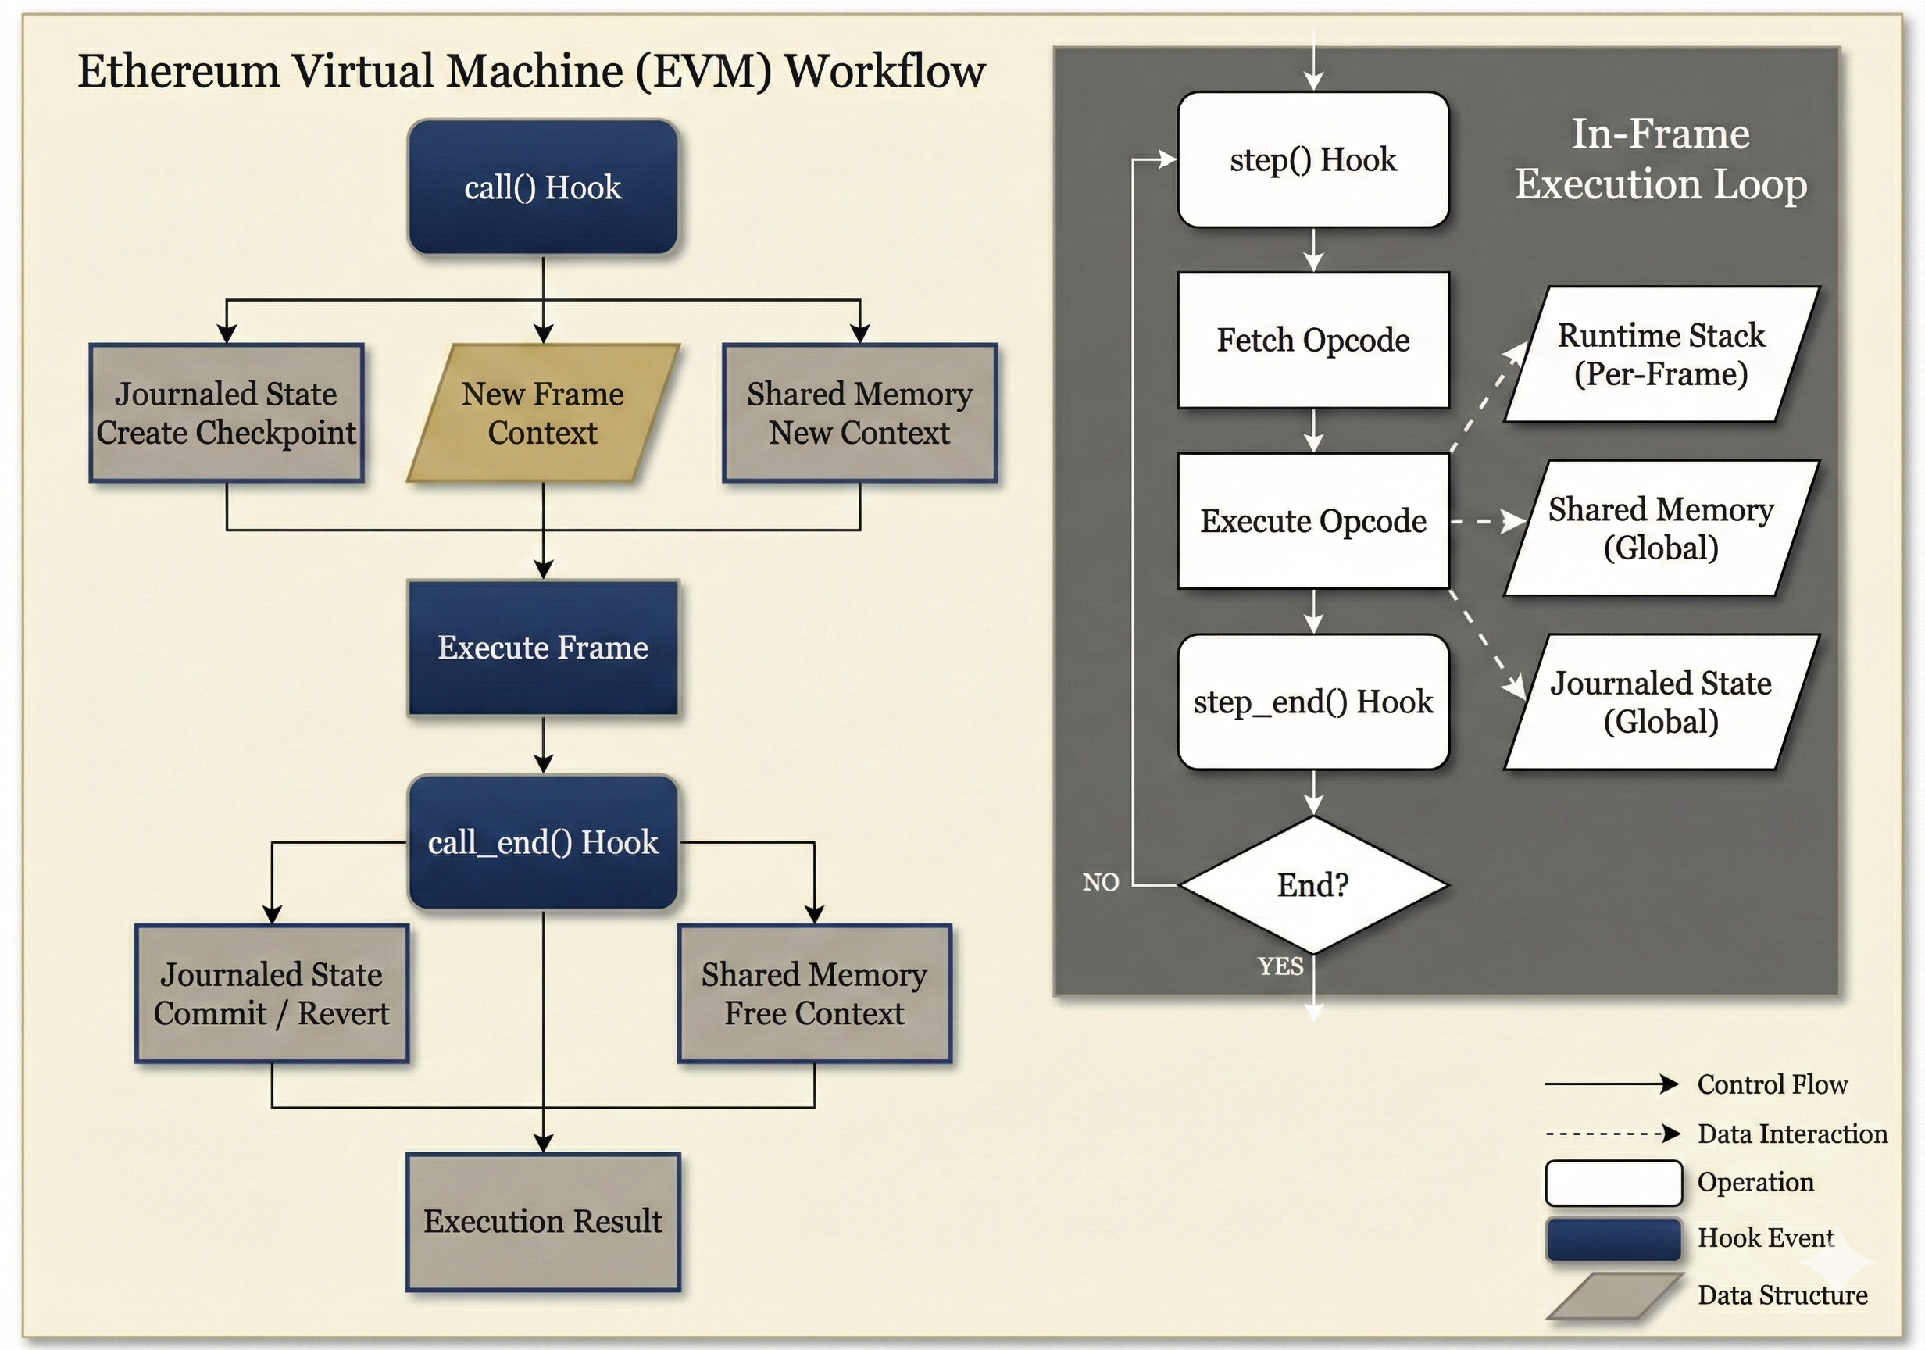
\includegraphics[width=\columnwidth]{raw-figures/EVM.drawio.pdf}
\caption{The EVM execution workflow. The process is partitioned into a high-level frame management lifecycle (left) and a low-level, per-opcode execution loop (right).}
\label{fig:evm-workflow}
\end{figure}


\subsection{The Ethereum Virtual Machine (EVM) Execution Model}
The EVM is a quasi-Turing-complete, stack-based virtual machine that serves as the sandboxed execution environment for smart contracts on the Ethereum blockchain. Its architecture and state model impose specific constraints and present unique opportunities for optimization, which directly inform the design of Helios. The overall execution workflow, depicted in Figure~\ref{fig:evm-workflow}, is partitioned into a high-level frame management lifecycle and a low-level, per-opcode execution loop. The following subsections detail the key components of this model.

\subsubsection{Stack-Based Architecture}
The EVM operates on a shared, 1024-element deep runtime stack where each element is a 256-bit word. All computational opcodes retrieve their operands by popping from the top of the stack and push their results back onto it. This model contrasts with traditional register-based architectures that operate on named registers via direct addressing. While conceptually simple, the stack-based design necessitates a high frequency of explicit stack manipulation instructions to manage data flow. These instructions, alongside the overhead of indirect memory access through a stack pointer, represent a primary target for optimization in Helios.

As illustrated in the in-frame execution loop of Figure~\ref{fig:evm-workflow}, every operation interacts with this per-frame runtime stack. Stack manipulation instructions, such as DUP1-DUP16 for duplicating items at various depths and SWAP1-SWAP16 for swapping the top element with items at different positions, are prevalent in EVM bytecode as compiler-generated boilerplate for managing operand placement. Unlike computational opcodes, these instructions rearrange existing stack elements without producing new values, making them particularly amenable to elimination.

\subsubsection{State Model: Volatile Memory and Persistent Storage}
The EVM maintains two distinct data storage mechanisms: transient memory and persistent storage, visually represented in Figure~\ref{fig:evm-workflow} as Shared Memory and Journaled State respectively. Memory is a byte-addressable linear array with transaction-scoped lifetime, utilized for ephemeral data such as function call arguments and intermediate computation buffers. Storage, by contrast, implements a persistent key-value mapping from 256-bit keys to 256-bit values, constituting the contract's global state that persists across transaction boundaries. Operations on storage are computationally more expensive than memory operations due to their impact on the global state.

The modification of memory and storage constitutes an observable side effect. This characteristic constrains compiler optimizations, as operations with such side effects cannot be reordered or eliminated without altering program semantics. Consequently, Helios focuses its most aggressive optimizations on the computational, side-effect-free operations that occur between state interactions.

\subsubsection{Call Frames}
EVM execution is organized into a hierarchy of call frames. The lifecycle of a single frame, from its creation to its finalization, is depicted in the workflow on the left side of Figure~\ref{fig:evm-workflow}. A new frame, with its own independent memory and runtime stack, is created for each function call, including external calls between different smart contracts. All frames within a single transaction, however, share access to the same persistent storage. A transaction's execution can thus be modeled as an ordered sequence of these call frames. 

\subsubsection{Hook Mechanism}
The EVM specification includes a standard hook mechanism to support native tracers and debuggers. This interface allows an external component to subscribe to events that are triggered immediately before and after the execution of each opcode, as well as at the entry and exit points of every call frame, which are explicitly marked as Hook Events in Figure~\ref{fig:evm-workflow}. This standard, non-invasive interface is foundational for any external profiling tool, as it enables the passive observation of an execution without modifying the core EVM interpreter.

\subsection{Gas: The Resource Metering Mechanism}
\label{sec:gas}
Gas is the fundamental mechanism in the EVM for metering computational resource consumption. It serves both to incentivize validators for the computational work they perform and to protect the network from denial-of-service attacks by ensuring that all executed operations are paid for.

Every transaction submitted to the network must specify a gas limit, representing the maximum amount of gas the originator is willing to consume. Each opcode executed by the EVM deducts a specific amount of gas from this limit. If the total gas consumed exceeds the limit at any point, the execution is halted, an out-of-gas (OOG) exception is raised, and all state changes made by the transaction are reverted. This mechanism ensures that even programs with infinite loops will eventually terminate, making the otherwise Turing-complete EVM a quasi-Turing-complete machine.

EVM gas costs can be categorized into two types: static and dynamic. Static costs are fixed, compile-time determinable values. The majority of opcodes, such as those for arithmetic or logical operations, have a low, constant gas cost. Dynamic costs are values that depend on the runtime state of the EVM. Examples include the cost of expanding memory, which is a quadratic function of the current memory size, or the cost of an SSTORE operation, which depends on whether a storage slot is being accessed for the first time in the transaction or has been accessed before.

This distinction is central to performance optimization, as it creates the opportunity to aggregate and pre-calculate the cumulative static gas costs of long instruction sequences. Dynamic costs, in contrast, must be calculated at runtime to ensure semantic equivalence.

Certain opcodes, termed gas delimiters, explicitly interact with the gas counter. On healthy execution paths where no out-of-gas exception occurs, these delimiters represent the only points where the gas balance must be observable. GAS reads the current gas balance onto the stack; RETURN, STOP, and REVERT finalize frame execution and require gas verification; CREATE and CREATE2 allocate gas to child contracts. These delimiters partition execution into segments, enabling bulk gas deduction for intervening operations.

\subsection{Node Types of the Ethereum Network}
The dual-mode design of Helios is a direct response to the distinct operational requirements and workload characteristics of the two primary types of nodes in the Ethereum network: Full Nodes and Archive Nodes.

A full node is responsible for participating in the real-time operation of the network. Its primary tasks include receiving new transactions from the peer-to-peer network, executing and validating them, and including them in new blocks. This workload is latency-sensitive, as block production times are fixed. Furthermore, full nodes must process transactions with limited predictability, as they frequently encounter novel smart contracts and previously unseen execution paths. This environment, characterized by low latency requirements and high uncertainty, motivates the need for an execution strategy that can perform on-demand, adaptive optimization as new transactions are observed.

An archive node stores the complete history of the blockchain's state from the genesis block to the present. Its primary workload involves serving historical data queries and, crucially, re-executing large batches of historical blocks, for instance, to sync a new node or for data analysis purposes. This workload is throughput-sensitive, prioritizing the total time to process millions of known, historical transactions over the latency of any single one. The execution is entirely deterministic, as the inputs and outcomes of all historical transactions are already recorded on the blockchain. This high-throughput, deterministic workload motivates the need for a specialized execution strategy that can leverage pre-computed knowledge of historical executions to achieve maximum speed with zero speculation overhead.

\subsection{Foundational Concepts in Code Optimization}
The design of Helios's SSA Optimizer is informed by foundational concepts from the field of compiler theory. A key concept is Static Single Assignment (SSA), an intermediate representation property where each variable is assigned a value exactly once. This property makes data dependencies explicit and simplifies a wide range of optimizations. An execution trace that assigns a unique identifier (e.g., a sequence number) to the result of every operation naturally produces an SSA-like representation. Additionally, the EVM ecosystem presents a clear opportunity for a caching system to implement a code/data separation strategy. Contract standards like ERC-20 result in thousands of deployed instances that share identical logic but differ only in their initial constant values, such as a token's name or total supply. With this background on the EVM's architecture, its resource metering model, and the operational context of blockchain nodes, we now proceed to motivate the design of Helios, addressing the limitations of existing approaches.

\subsection{Prior EVM Optimization Approaches}
Recent systems have explored path-driven optimization strategies to accelerate EVM execution. Forerunner~\cite{forerunner} employs constraint-based speculative execution, pre-executing transactions in the transaction pool and generating optimized fast-path programs guarded by control-flow and data-dependency constraints. Seer~\cite{seer} introduces fine-grained branch prediction with checkpoint-based snapshots to maximize pre-execution result reuse across different execution paths. ParallelEVM~\cite{parallelEvm} achieves operation-level concurrent transaction execution through SSA-based conflict detection and selective re-execution of conflicting operations. EVMTracer~\cite{evmTracer} provides dynamic analysis tools to construct opcode-level dependency graphs for quantifying parallelization potential and computational redundancy.

These systems employ comprehensive tracing mechanisms that capture complete execution state, including stack operations, memory accesses, and storage dependencies, enabling detailed analysis and optimization of execution paths across EVM-compatible blockchain systems.
\section{Motivation}

Traditional path-driven optimization systems like Forerunner and Seer achieve 5–8× speedups on classical EVM interpreters such as Geth. However, when applied to modern, highly-optimized implementations like Revm, these gains diminish sharply. For identical bytecode, speedups drop from 5.0× on Geth to only 1.5× on Revm. This degradation exposes fundamental limitations in existing optimization strategies when baseline execution is already fast. Through systematic analysis across four critical design dimensions of optimization paradigm, tracing strategy, artifact organization, and correctness guarantees, we derive a set of principled design choices that enable effective optimization on modern EVMs. Each choice addresses specific bottlenecks while establishing constraints that guide subsequent decisions, ultimately converging on Helios's architecture.

% requires listing subcaption and amssymb

\begin{figure*}[t]
\centering
\begin{subfigure}[t]{0.48\textwidth}
\begin{lstlisting}[
  language=,
  basicstyle=\scriptsize\ttfamily,
  numbers=left,
  numberstyle=\tiny\color{gray},
  xleftmargin=3em,
  framexleftmargin=2.5em,
  frame=single
]
PUSH1 0x05
JUMPDEST          // loop_start
DUP1
ISZERO
PUSH1 loop_end
JUMPI
  PUSH1 0x01
  SLOAD
  POP
  PUSH1 0x01
  SWAP1
  SUB
PUSH1 loop_start
JUMP
JUMPDEST          // loop_end
POP
\end{lstlisting}
\caption{Native execution: 2500 gas}
\label{fig:native-loop}
\end{subfigure}
\hfill
\begin{subfigure}[t]{0.48\textwidth}
\begin{lstlisting}[
  language=,
  basicstyle=\scriptsize\ttfamily,
  numbers=left,
  numberstyle=\tiny\color{gray},
  xleftmargin=3em,
  framexleftmargin=2.5em,
  frame=single
]
PUSH1 0x01
SLOAD             // loop hoisting
POP
PUSH1 0x05
JUMPDEST          // loop_start
DUP1
ISZERO
PUSH1 loop_end
JUMPI
  PUSH1 0x01
  SWAP1
  SUB
PUSH1 loop_start
JUMP
JUMPDEST          // loop_end
POP
\end{lstlisting}
\caption{After loop hoisting: 2100 gas}
\label{fig:hoisted-loop}
\end{subfigure}
\caption{Loop hoisting optimization violates gas-semantic equivalence. Native execution (a) performs 5 storage reads of slot 0x01 (lines 7--8 in loop body): the first SLOAD incurs a cold read cost of 2100 gas under EIP-2929, while subsequent iterations pay 100 gas each for warm reads, totaling $2100 + 4 \times 100 = 2500$ gas. JIT optimization (b) detects that SLOAD(0x01) is loop-invariant and hoists it outside the loop (lines 2--3), reducing execution to a single storage read consuming only 2100 gas. This 400-gas divergence violates gas-semantic equivalence, creating economic misalignment: charging the original 2500 gas overcompensates miners for actual resource usage, while charging only 2100 gas undercompensates them.}
\label{fig:loop-hoisting-gas}
\end{figure*}

\subsection{Path-Driven over Contract-Driven Optimization}
\label{sec:path-vs-contract}
EVM optimization can follow two competing paradigms. Contract-driven optimization, exemplified by JIT compilation approaches, optimizes entire contracts. Path-driven optimization, employed by systems like Forerunner and Seer, optimizes only executed traces. This foundational choice establishes the scope and safety model for all subsequent design decisions.

Contract-driven approaches compile entire contract bytecode into optimized native code, enabling aggressive global optimizations such as loop hoisting, dead code elimination, and cross-basic-block register allocation. These transformations can yield substantial performance improvements on hot contracts. However, this paradigm faces two critical challenges in production blockchain environments.

First, unrestricted JIT compilation introduces severe security risks through JIT Bomb attacks. Malicious bytecode can exploit compilation complexity by using deeply nested control flow or pathological loop structures to force the JIT compiler into exponential-time compilation or excessive memory consumption. This denial-of-service vector is particularly dangerous in blockchain contexts where attackers can trivially deploy adversarial contracts and force validators to compile them. Existing JIT-based EVM implementations address this threat through contract whitelisting, restricting optimization to pre-approved contracts. This mitigation severely limits applicability, as the majority of contract invocations fall outside whitelists, rendering the optimization ineffective for general workloads.

Second, aggressive global optimizations frequently violate gas-semantic equivalence. Figure~\ref{fig:loop-hoisting-gas} illustrates this problem through a representative example where loop hoisting reduces the number of storage reads, thereby changing the gas consumption profile. While this transformation improves performance, it creates economic misalignment between charged fees and actual resource usage. This divergence presents validators with an undesirable choice between overcompensating for work performed or undercompensating relative to network standards, potentially discouraging adoption of the optimization.

Path-driven optimization offers a different trade-off. By optimizing only actually-executed paths rather than entire contracts, this paradigm inherently bounds optimization costs per path, eliminating JIT Bomb vulnerabilities. Every path processed represents real execution that already occurred, ensuring compilation work scales linearly with actual usage rather than potential attack surface. This enables universal deployment without whitelists. Any contract invoking frequently-executed paths automatically benefits from optimization, regardless of bytecode complexity or origin.

However, path-driven systems must still address gas-semantic preservation explicitly. While this paradigm avoids the cross-contract global optimizations that complicate gas preservation in JIT approaches, it does not automatically guarantee gas equivalence. Existing path-driven systems such as Forerunner and Seer do not explicitly discuss this equivalence in their design. Helios achieves precise gas-semantic preservation through specific design choices, particularly the combination of stack-only tracing, frame-level organization, and path-local transformations, as we will demonstrate in \S\ref{sec:gas-semantic-equivalence}.

The choice of path-driven optimization establishes our first architectural constraint. We optimize execution traces post-facto rather than contracts a priori. This decision prioritizes safety and universal applicability over maximal theoretical performance, setting the foundation for subsequent design choices.

% require \usepackage{booktabs}
\begin{table}[t]
\centering
\caption{Performance degradation of path-driven optimization on modern EVMs. 
Measurements on Uniswap V2 swap (1-hop) demonstrate that artifact overhead 
dominates when baseline execution is fast.}
\label{tab:motivation-overhead}
\small
\resizebox{\columnwidth}{!}{%
\begin{tabular}{llrrr}
\toprule
\textbf{System} & \textbf{Client} & \textbf{Latency} & \textbf{Speedup} & \textbf{Artifact} \\
 & & \textbf{(µs)} & \textbf{(×)} & \textbf{(KB)} \\
\midrule
Native          & Geth         & 398.4   & 1.0×    & --    \\
Forerunner      & Geth         & 68.1    & 5.8×    & 910   \\
\midrule
Native          & Revm         & 62.0    & 1.0×    & --    \\
Forerunner      & Revm         & 39.2    & 1.6×    & 663   \\
\midrule
\textbf{Helios} & \textbf{Revm} & \textbf{31.0} & \textbf{2.0×} & \textbf{70} \\
\bottomrule
\end{tabular}%
}
\end{table}

\subsection{The Overhead of Existing Path-Driven Approaches}
Having established the path-driven paradigm, we now examine why existing implementations struggle on modern EVMs. The core issue is a performance paradox. Detailed tracing, once a minor cost on slow interpreters, becomes the primary bottleneck when baseline execution is already fast.

This paradox manifests most severely in the memory I/O cost of optimization artifacts. Table~\ref{tab:motivation-overhead} demonstrates this performance degradation through measurements on a representative Uniswap V2 single-hop swap. Forerunner achieves substantial speedups on Geth but experiences diminished returns on Revm despite generating identical 663 KB trace artifacts. We note that since Forerunner does not provide a native Revm implementation, our measurements employ a functionally equivalent mock implementation that replicates Forerunner's tracing and optimization strategy on the Revm runtime. The reduced baseline execution time on modern EVMs exposes artifact overhead as the dominant bottleneck. When baseline execution completes in tens of microseconds, loading and parsing trace artifacts of this magnitude consumes time comparable to the computational work being optimized.

However, artifact I/O represents only part of the overhead. Full-tracing approaches that maintain custom execution context management—including call frames, memory snapshots, and storage deltas—forgo the host EVM's optimized native implementations. For complex transactions with artifacts exceeding hundreds of kilobytes, I/O latency dominates. For simple transactions such as ERC20 transfers, where artifact sizes remain modest, the computational cost of redundant context management becomes the primary bottleneck. Modern EVMs provide highly optimized frame-level infrastructure. An effective strategy must leverage these mechanisms rather than duplicating them.

Tracing itself also introduces computational overhead. Existing systems employ different strategies to mitigate this cost. Forerunner and Seer perform tracing in the transaction pool, asynchronously profiling pending transactions before block execution. This removes tracing from the critical path, though artifact I/O costs remain during actual execution. ParallelEVM performs online tracing during parallel execution, where each thread simultaneously executes and traces transactions before resolving conflicts through selective re-execution. This strategy reduces memory I/O by avoiding large pre-generated artifacts and relying instead on runtime dependency tracking.

However, on modern EVMs like Revm, both strategies become prohibitively expensive. We instrumented Revm with a comprehensive tracer recording stack, memory, and storage dependencies during execution. Single-transaction latency increased from 60 µs to over 300 µs, representing a 5× slowdown on the critical path. This overhead stems from per-opcode hook invocations, shadow data structure maintenance, and context switches between the EVM engine and tracing infrastructure. When baseline execution operates at this speed, these mechanisms consume time comparable to the operations being traced.

Furthermore, the purported advantage of full dependency tracking proves illusory in practice. EVMTracer proposed exploiting opcode-level dependencies to parallelize execution within a single transaction. We implemented a dependency-graph-driven parallel executor for Revm that schedules independent opcodes across multiple threads based on recorded dependencies. Contrary to theoretical models, the parallel version consistently underperformed its optimized serial counterpart. The root cause is fundamental. At nanosecond execution granularity, thread synchronization and communication overhead far exceeds the time saved by parallel instruction execution. When individual opcodes complete in 20 nanoseconds but thread coordination requires hundreds of nanoseconds, parallelism merely adds overhead.

\noindent\textbf{Design Principle 1.} \emph{Minimize analysis overhead through lightweight, asynchronous tracing that leverages host EVM infrastructure.} To achieve meaningful speedups on modern EVMs, an optimization strategy must produce compact artifacts to minimize I/O costs, operate asynchronously off the critical execution path, reuse the host EVM's optimized frame management and state access mechanisms, and capture only information that enables practical, low-overhead optimizations.

This principle establishes the next constraint. Any tracing mechanism must be selective, focusing on the subset of execution state that yields the highest optimization return per byte of trace data. The question then becomes what subset of execution dependencies we should capture.

\subsection{Frame-Level Reuse over Monolithic Traces}
\label{sec:frame-level-caching}

\begin{figure}[b]
\centering
\includegraphics[width=\columnwidth]{raw-figures/pareto_cumulative.pdf}
\caption{Path locality in EVM execution follows an extreme Pareto distribution: the top 1\% of unique paths account for 70\% of frame executions (5,000 mainnet blocks). The shaded region shows deviation from uniform distribution.}
\label{fig:pareto-cumulative}
\end{figure}

The previous section established the need for lightweight tracing. However, reducing tracing overhead alone is insufficient. We must also maximize the value extracted from each traced execution. This requires addressing two interrelated design decisions regarding the granularity of optimization artifacts and the mechanisms for enabling their reuse across transactions.

Existing path-driven systems adopt transaction-level artifact organization, where each transaction's optimization artifacts are generated and discarded immediately after use. This granularity choice introduces severe limitations for reuse. Consider three transactions where Tx1 calls contracts C1→C2, Tx2 calls C3→C4, and Tx3 calls C1→C3. Under transaction-level organization, Tx3 cannot reuse cached artifacts from Tx1 or Tx2, despite sharing individual contract call frames. The cache key is the entire transaction's execution pattern, the specific sequence C1→C3, rather than individual frame paths. Even though the C1 invocation in Tx3 may be identical to the C1 invocation in Tx1, and the C3 invocation identical to that in Tx2, the system is forced to retrace both frames because the transaction-level composition is novel. This use-once-discard model represents significant wasted effort. Even when constituent frames execute along identical paths, the system repeats the full tracing and optimization process.

Frame-level organization resolves this limitation by treating each contract call frame as an independent optimization unit. In the Tx3 example, the individual C1 frame can be recognized and reused from Tx1's cache, and the C3 frame from Tx2's cache. Only genuinely novel frame-level execution patterns require new tracing. This compositional reuse substantially increases effective cache coverage. Rather than requiring exact transaction-level matches, the system benefits from any partial overlap in the frame-level call graph.

To validate this design choice and quantify the economic value of frame-level caching, we conducted large-scale path analysis on Ethereum mainnet blocks 19,600,000 through 19,605,000. For each contract call frame, we compute a path identifier by hashing the sequence of executed opcodes within that frame, then track the frequency distribution of these unique path identifiers across all frames in the analyzed blocks.

The results in Figure~\ref{fig:pareto-cumulative} reveal a pronounced Pareto distribution with strong path locality. The top 10\% of unique paths account for over 90\% of all frame executions. Further decomposition shows extreme concentration. The top 1\% of paths handle 70\% of executions, and the top 5\% handle 85\%. This distribution remains stable across different block ranges and time periods, indicating that path locality is a fundamental characteristic of EVM execution rather than transient behavior.

This empirical finding confirms the value of persistent, frame-level caching. For high-frequency paths in the top 1\%, a single tracing cost can be amortized across hundreds or thousands of subsequent executions. When a path appears 1000 times but requires tracing only once, the effective per-execution overhead becomes negligible, fundamentally changing the cost-benefit ratio compared to transaction-level use-once-discard approaches. The extreme concentration further suggests that even modest cache sizes can achieve high hit rates by retaining only the most frequently executed paths.

Furthermore, frame-level granularity aligns naturally with the EVM's execution model, which inherently manages resources and state at frame boundaries. Each call frame operates within an isolated context with its own memory space, storage view, and gas quota. This alignment allows direct reuse of mature frame management infrastructure from host EVM clients, including optimized memory allocation and storage access patterns. Transaction-level approaches, by contrast, must implement custom frame simulation logic to maintain correctness across artificially flattened execution sequences, adding complexity and potential correctness risks.

The combination of empirical path locality and architectural alignment motivates our second principle.

\noindent\textbf{Design Principle 2.} \emph{Enable cross-transaction reuse through frame-level, persistent caching.} Optimization artifacts should be organized at the frame granularity and indexed by per-frame path identifiers. This enables compositional reuse across transactions, amortizes optimization costs across high-frequency paths, and leverages host EVM infrastructure for frame management.

This principle establishes two additional constraints. First, artifact organization must respect frame boundaries. Second, caching must support persistent storage with efficient lookup. These constraints, combined with the lightweight tracing requirement from Principle 1, narrow the design space considerably. The remaining question is what specific execution information we should trace and optimize.

\subsection{Achieving Natural Gas-Semantic Equivalence}
\label{sec:gas-semantic-equivalence}

The previous sections established the need for lightweight, frame-level, path-driven optimization. However, any optimization strategy must ultimately satisfy a critical correctness requirement specific to blockchain execution. Exact preservation of gas semantics is essential because gas underpins miner incentives in Ethereum's economic model. Transaction senders pay fees proportional to gas consumed. Any optimization altering gas consumption disrupts this economic balance, either overcompensating miners when charging original gas for reduced work or undercompensating them when charging reduced gas. Maintaining gas-semantic equivalence, defined as exact matching of native execution's gas accounting, is thus an economic necessity for practical adoption.

The core challenge stems from the distinction between static-cost and dynamic-cost instructions as defined in \S\ref{sec:gas}. Static-cost instructions have compile-time-determinable gas costs, while dynamic-cost instructions have runtime-dependent costs that depend on state such as memory expansion or storage access history.

Any optimization that eliminates or reorders dynamic-cost instructions risks gas divergence, as demonstrated in \S\ref{sec:path-vs-contract} with loop hoisting. However, if we restrict optimization to static-cost instructions only, gas preservation becomes straightforward. We precompute the cumulative gas of eliminated operations and deduct it in bulk, while ensuring all dynamic-cost instructions execute natively with precise accounting.

Remarkably, our previous design decisions, driven by entirely orthogonal concerns, naturally converge to enable this strategy. First, lightweight tracing from Principle 1 led us to focus on operations with low tracing overhead while excluding those requiring substantial state tracking. This scope restriction carries an important secondary consequence. Operations excluded due to tracing cost are precisely those with dynamic gas pricing, such as memory expansion and storage access history, while the traced operations are precisely those with static costs. The excluded instructions also share a common characteristic. They perform side effects on persistent or expandable state, making their costs inherently runtime-dependent. In contrast, the included instructions operate solely on the evaluation stack, a fixed-size structure whose manipulation incurs predictable, compile-time-determinable costs.

Second, frame-level granularity from Principle 2 aligns optimization boundaries with the EVM's native gas accounting boundaries, as each call frame independently tracks gas consumption. Third, the path-driven paradigm from \S\ref{sec:path-vs-contract} constrains optimization to path-local transformations, avoiding cross-basic-block optimizations that would complicate gas accounting across control flow.

The convergence of these three orthogonal choices produces an elegant emergent property. Lightweight tracing naturally selects static-cost operations, frame-level organization aligns with gas boundaries, and path-driven optimization constrains transformations. Together, the optimization scope naturally excludes all dynamic-cost, side-effecting instructions, enabling gas-semantic equivalence without compensatory mechanisms. Each decision, motivated by distinct concerns of overhead reduction, reuse efficiency, and security, contributes guarantees that combine to solve the correctness problem. This is not a coincidence requiring delicate engineering but a robust consequence of constraint composition.

This convergence motivates our third principle.

\noindent\textbf{Design Principle 3.} \emph{Achieve gas-semantic equivalence as an emergent property of design constraints.} By restricting optimization to static-cost instructions through stack-only tracing, aligning artifact boundaries with gas accounting boundaries through frame-level organization, and constraining transformations through path-driven optimization, gas preservation arises naturally. The system can freely optimize within this scope without trading off performance against correctness.

\subsection{Synthesis: Deriving the Helios Architecture}
\label{sec:synthesis}

The three design principles of lightweight asynchronous tracing, frame-level persistent caching, and emergent gas-semantic equivalence map to Helios's architectural components with varying directness. The first two principles directly drive core components, while the third principle emerges as a natural consequence of their interaction.

Principle 1 manifests in three functional requirements. First, a selective tracer must capture execution dependencies with minimal overhead, generating compact artifacts approximately one order of magnitude smaller than full traces. Second, an asynchronous processing pipeline must decouple tracing from execution, processing artifacts off the critical path through background threads to eliminate online overhead while maintaining low artifact availability latency. Third, the tracing mechanism must leverage the host EVM's optimized native infrastructure for frame management and state access.

Principle 2 necessitates a persistent caching mechanism with per-frame-path indexing. The cache must support both deterministic lookup for known path identifiers and speculative querying for predicted hot paths. Persistent storage enables cross-transaction amortization. High-frequency paths in the top 1\% incur tracing costs once but benefit thousands of subsequent executions. Frame-level granularity enables compositional reuse, as demonstrated in \S\ref{sec:frame-level-caching}, substantially increasing effective cache coverage compared to transaction-level approaches.

An efficient execution engine is required to consume cached artifacts and accelerate hot path execution. This engine must translate traced execution sequences into an optimized execution model while preserving correctness. Principle 3 constrains the optimization scope to naturally exclude dynamic-cost operations, enabling a straightforward gas accounting strategy. The system precomputes cumulative static gas for optimized operations and deducts it in bulk at frame entry, while delegating all excluded dynamic-cost operations to the native mechanism. This design achieves exact gas equivalence without runtime compensation logic or gas recalculation overhead.

These components support two operational modes addressing distinct node workloads. Replay Mode targets archive nodes performing deterministic historical synchronization. Since all execution paths are known and unchanging, the cache can be pre-populated through one-time tracing of the entire blockchain history. Subsequent replays achieve complete cache coverage, amortizing single tracing costs across thousands of re-executions and enabling substantial speedups with minimal storage overhead, making historical replay economically viable for resource-constrained archive nodes.

Online Mode addresses full nodes processing unpredictable live transactions. Background tracing captures new paths without blocking execution per Principle 1. Dynamic caching maintains coverage of hot paths while evicting cold ones under memory pressure per Principle 2. When a cached path is available, the system executes it optimistically. On cache misses or validation failures, execution falls back to native interpretation, ensuring correctness for never-before-seen patterns.

Critically, both modes share identical core components and artifact formats, differing only in cache population strategy and execution strategy. Pre-fill versus on-demand caching distinguishes Replay Mode from Online Mode, as does deterministic versus speculative execution. This unified design allows a single implementation to span the full node-type spectrum. Quantitative performance evaluation, including detailed speedup measurements, cache hit rates, and storage overhead analysis for both operational modes across diverse workloads, is presented in \S\ref{sec:evaluation}.

Building on these three design principles and their instantiation across operational scenarios, the following section presents Helios's detailed architecture.
\section{The Design of Helios}
\label{sec:design}

\subsection{Overview}
Helios is a path-driven execution engine designed to accelerate EVM transaction processing. Its architecture comprises four coordinated components. The Helios Engine orchestrates execution. The Path Cache indexes optimized graphs for reuse. The Path Tracer captures execution traces. The SSA Optimizer compiles them into an optimized intermediate representation. Figure~\ref{fig:helios-architecture} illustrates the system architecture and data flow.

\begin{figure}[!htbp]
    \centering
    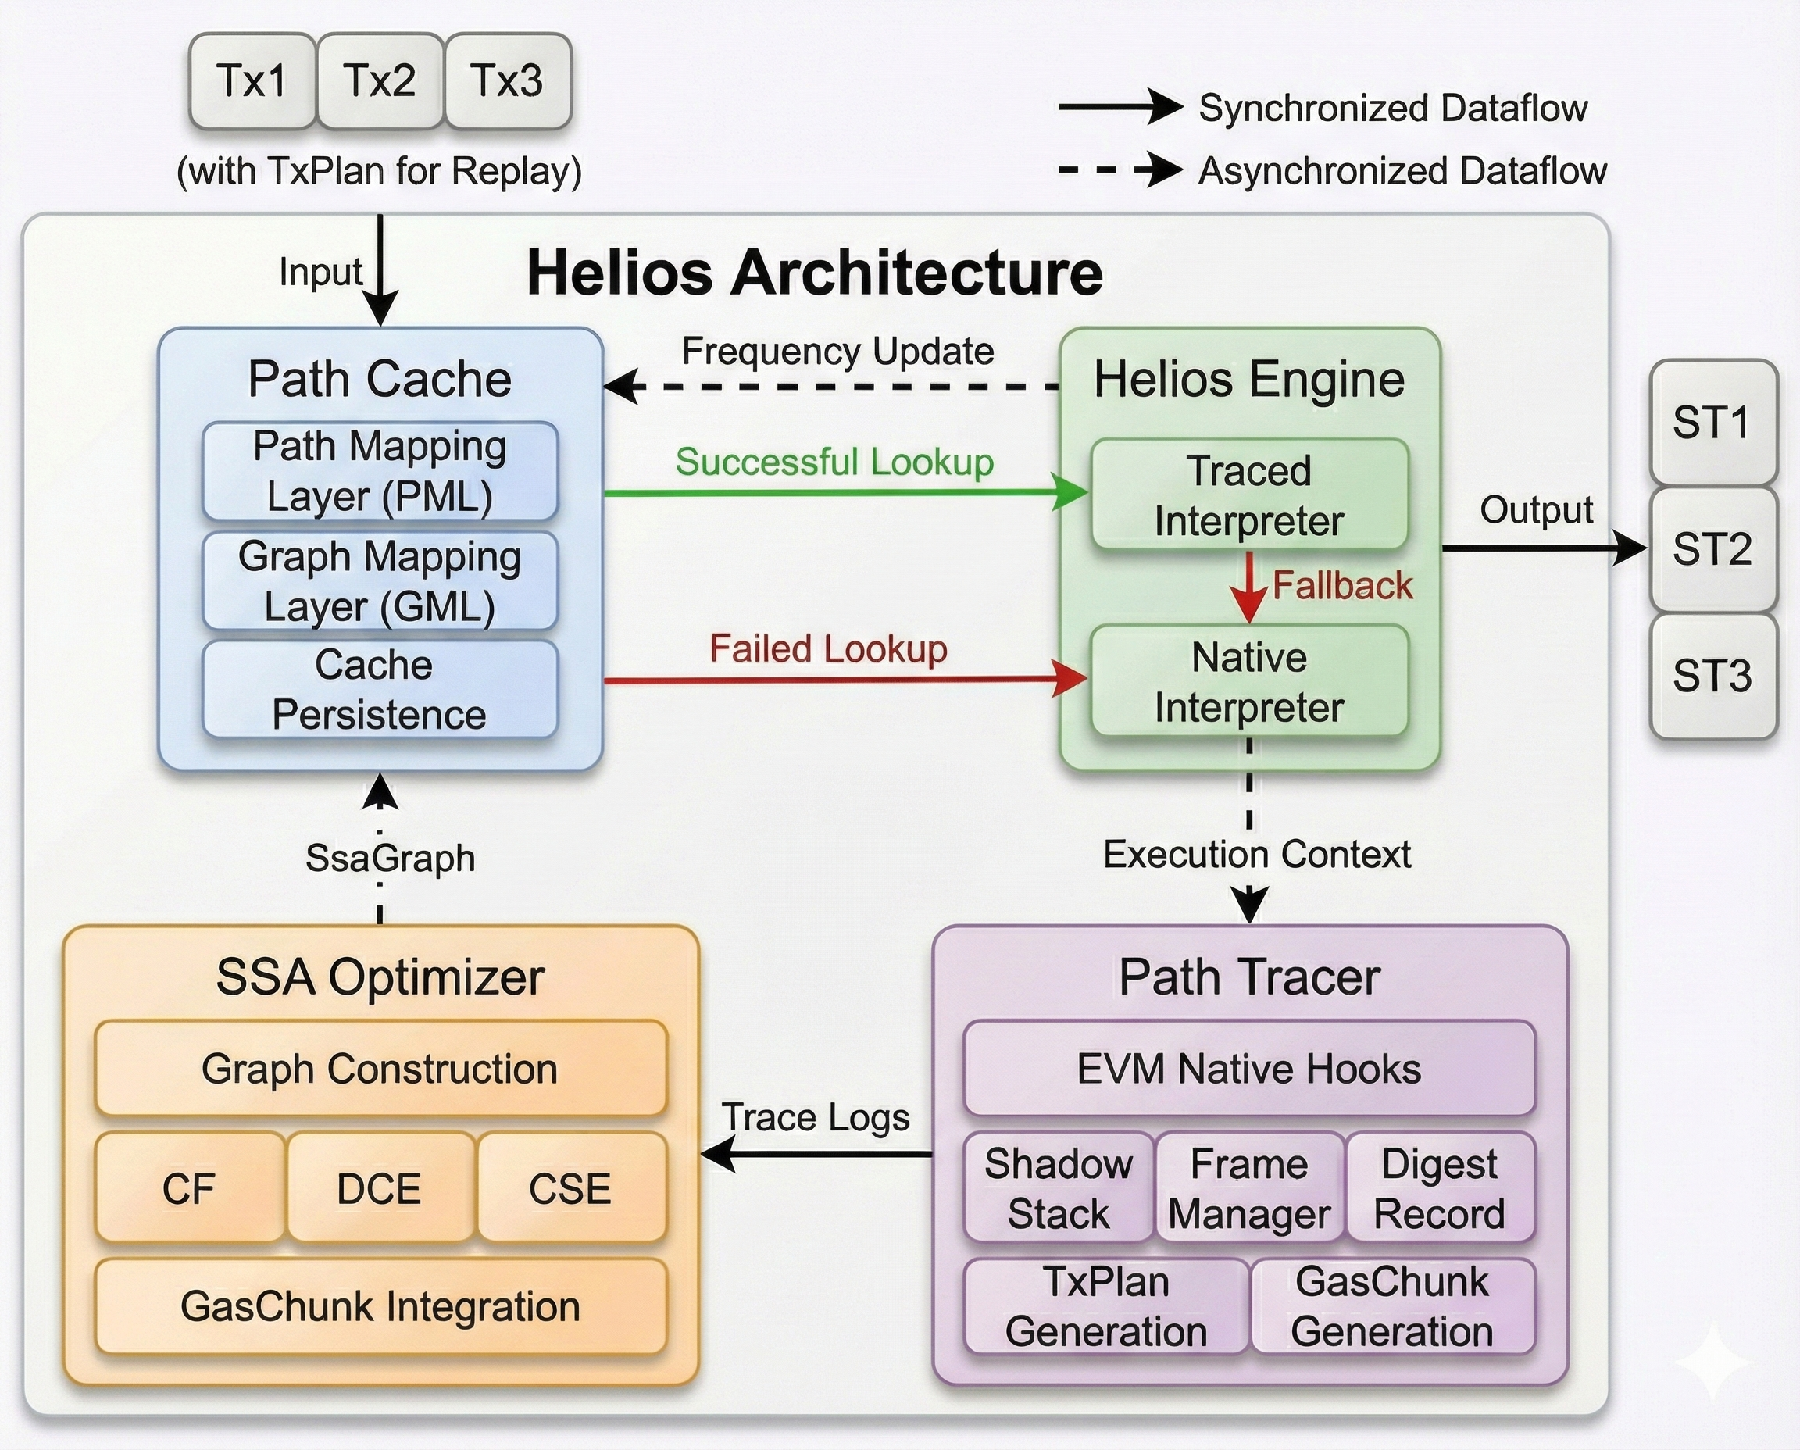
\includegraphics[width=\linewidth]{raw-figures/helios-architecture.pdf}
    \caption{Overview of the Helios architecture.}
    \label{fig:helios-architecture}
\end{figure}

Upon contract invocation, the Helios Engine queries the Path Cache using a path identifier derived from the contract identity and call signature. On a cache miss, the engine delegates execution to the Native Interpreter. This delegation simultaneously initiates an asynchronous optimization pipeline. The Path Tracer captures the raw execution trace as a PathLog, a linear sequence of executed opcodes with their data dependencies. The SSA Optimizer transforms this PathLog into an optimized SsaGraph, a directed acyclic graph that makes data flow explicit. The Path Cache then stores the SsaGraph for future reuse. Running in parallel with the Native Interpreter, this pipeline ensures that optimization never blocks the critical execution path.

On a cache hit, the engine retrieves the corresponding SsaGraph and dispatches it to the Traced Interpreter, which performs speculative execution validated by runtime control-flow guards. An execution failure triggers a fallback to the Native Interpreter and re-initiates the optimization pipeline. Successful execution concludes the transaction with reduced overhead.

Helios supports two operational modes. Online mode targets full nodes and validators handling transactions with unknown paths, where cache misses and guard failures may occur. Replay mode targets archive nodes reprocessing historical blocks. A pre-computed TxPlan guarantees cache hits for every call frame, allowing the engine to bypass control-flow guards and the optimization pipeline for maximum throughput.


\subsection{Key Data Structures}
Helios represents and indexes transaction paths through a small set of data abstractions that govern both Online and Replay modes.

\textbf{Path Representation.}
Execution paths are first captured as a \textit{PathLog}, a raw linear trace produced by the Path Tracer. A PathLog is a sequence of entries, each recording an opcode together with its stack data dependencies, expressed as references to the outputs of preceding operations. The optimization pipeline consumes this representation and transforms it into an \textit{SsaGraph}, a directed acyclic graph whose nodes denote operations and whose edges denote data dependencies. By making data flow explicit and eliminating the implicit EVM stack, the SsaGraph serves as the executable format for the Traced Interpreter.

\textbf{Path Indexing and Retrieval.}
Helios employs a multi-key scheme to locate and reuse SsaGraphs. A \textit{PathDigest} is a 64-bit hash of a path’s opcode sequence acting as a deterministic identifier for the execution logic. A \textit{DataKey} concatenates a contract’s code hash with the PathDigest to uniquely identify the constant table for a specific contract instance. This separation allows multiple contracts with identical bytecode, such as distinct ERC20~\cite{erc20} tokens, to share a single SsaGraph while maintaining separate constant tables. Finally, a \textit{CallSig} is a coarse-grained identifier used for predictive lookup in Online mode, defined as the concatenation of a contract’s code hash and the 4-byte function selector from calldata. A single CallSig may map to multiple PathDigests, corresponding to distinct control-flow branches of the same function, including both successful and revert paths.

\textbf{Execution Metadata.}
Helios maintains additional metadata to coordinate cross-frame execution and reduce runtime overhead. A \textit{Transaction Plan (TxPlan)} is an ordered sequence of PathDigests that records the path taken by each call frame within a transaction. TxPlans are produced during Online execution and indexed by block number and transaction index; in Replay mode, they provide a deterministic guide for fetching the correct SsaGraph for every frame. A \textit{GasChunk} is a precomputed scalar capturing the cumulative static gas cost of the instructions lying between two consecutive gas-accounting opcodes. Attached to the corresponding SsaGraph, GasChunks allow the Traced Interpreter to replace per-instruction gas accounting with a single bulk deduction, thereby reducing overhead while preserving gas-semantic equivalence.

\subsection{Component Design and Implementation}
This section details the internal design and mechanisms of each of Helios's four primary components. It describes how each component fulfills its role in the end-to-end transaction lifecycle, transforming its inputs into the data structures required by the next stage of the pipeline.


\begin{algorithm}[!htbp]
\small
\caption{Shadow Stack Tracing}
\label{alg:shadow-stack-tracing}
\KwIn{$op$: Current EVM opcode}
\KwIn{$S_{evm}$: EVM value stack (after opcode execution)}
\KwIn{$S_{\ell}$: Shadow stack of LSNs tracking value provenance}
\KwOut{$e$: Trace log entry containing the opcode, current LSN, input dependencies, and output value}
\KwOut{Updated $S_{\ell}$}

\tcp{Extract input dependencies from shadow stack}
$D_{in} \gets []$ \\
$k \gets$ \textsc{GetInputCount}$(op)$ \\
\For{$i \gets 1$ \KwTo $k$}{
    $\ell \gets S_{\ell}$.\textsc{Pop}() \\
    $D_{in}$.\textsc{Append}$(\ell)$ \\
}

\tcp{Record output value and assign new LSN}
\eIf{$op$ produces stack output}{
    $v_{out} \gets S_{evm}$.\textsc{Top}() \\
    $\ell_{curr} \gets$ \textsc{NextLSN}() \\
    $S_{\ell}$.\textsc{Push}$(\ell_{curr})$ \\
}{
    $v_{out} \gets \bot$ \tcp*{No output, e.g., POP, JUMP}
    $\ell_{curr} \gets$ \textsc{NextLSN}() \\
}

\tcp{Handle stack manipulation instructions}
\If{$op \in \{\text{\texttt{DUP1}}, \text{\texttt{DUP2}}, \ldots, \text{\texttt{DUP16}}\}$}{
    $d \gets op - \text{\texttt{DUP1}} + 1$ \\
    $\ell_t \gets S_{\ell}[d]$ \tcp*{Peek without pop}
    $S_{\ell}$.\textsc{Push}$(\ell_t)$ \tcp*{Duplicate LSN}
}
\If{$op \in \{\text{\texttt{SWAP1}}, \text{\texttt{SWAP2}}, \ldots, \text{\texttt{SWAP16}}\}$}{
    $d \gets op - \text{\texttt{SWAP1}} + 1$ \\
    $S_{\ell}$.\textsc{Swap}$(0, d)$ \tcp*{Swap LSNs}
}

\tcp{Create log entry}
$e \gets \langle op, \ell_{curr}, D_{in}, v_{out} \rangle$ \\

\Return{$e$}

\end{algorithm}

\subsubsection{Path Tracer}
A lightweight instrumentation component observes native EVM execution to produce the raw PathLog data structure, TxPlan, and GasChunk.

\textbf{Instrumentation mechanism.} The tracer attaches to the EVM hook interface and subscribes to six events, including \texttt{step} and \texttt{step\_end} for opcode execution, \texttt{call} and \texttt{call\_end} for external calls, and \texttt{create} and \texttt{create\_end} for contract creation. This hook-based design decouples the tracer from the interpreter and enables passive observation without changing execution semantics.

To capture stack data dependencies, the tracer maintains a shadow stack mirroring the EVM operand stack but storing 32-bit Log Sequence Numbers or LSNs instead of 256-bit values. Each LSN identifies the operation producing the corresponding value. As detailed in Algorithm~\ref{alg:shadow-stack-tracing}, the tracer pops the required input LSNs to form the dependency list $D_{in}$ on each \texttt{step\_end}, allocates a new LSN for the current opcode, and pushes it if the opcode produces a stack result. For stack-manipulation opcodes such as \texttt{DUP} and \texttt{SWAP} that only reorder values, the tracer applies the same permutation to the shadow stack without creating a new LSN. As a result, only opcodes that actually produce new values become nodes in the PathLog, effectively collapsing substantial stack traffic and yielding PathLog entries that record each operation alongside the LSNs of its true data dependencies.

\textbf{PathDigest Calculation.} PathDigest is a rolling hash updated with each executed opcode using the lightweight FNV-1A algorithm~\cite{fnv1, fnv2}. FNV-1A was chosen for its efficiency, involving simple multiplication and XOR operations. This ensures a unique identifier for each execution path and allows fast incremental updates, enabling efficient path comparison and lookup in the PathCache.

\textbf{Metadata generation.} The tracer also constructs GasChunk and TxPlan metadata. For GasChunks, it treats \texttt{GAS} and terminating opcodes such as \texttt{RETURN}, \texttt{STOP}, \texttt{REVERT}, \texttt{CREATE}, and \texttt{CREATE2} as gas delimiters. It accumulates the static gas cost of instructions between two delimiters and emits a GasChunk with the aggregate cost upon reaching a delimiter. If a path ends without an explicit delimiter, the system inserts a synthetic \texttt{STOP} to close the final chunk.

The TxPlan is built using placeholders. When a new frame is entered via the \texttt{call} or \texttt{create} hook, the tracer appends a placeholder entry. When the frame completes at \texttt{call\_end} or \texttt{create\_end}, it computes the frame's PathDigest and replaces the placeholder. The resulting TxPlan records the final per-frame path sequence in transaction order.

\textbf{Path Validation and Filtering.} To restrict resource allocation to reusable paths, the tracer executes a health check during the \texttt{call\_end} hook by inspecting the frame's exit status. The system discards paths resulting from VM-level exceptions, particularly out-of-gas errors, while retaining deterministic application-level terminations such as successful returns and \texttt{REVERT} operations. This distinction is critical because \texttt{REVERT} paths correspond to reproducible control-flow branches, including failed assertions or balance validations, which exhibit high reusability across transactions. Conversely, VM-level exceptions are non-deterministic and may manifest at any instruction depending on the gas limit. Tracking every potential out-of-gas point for a sequence of $n$ opcodes would generate $O(n)$ distinct failure paths, leading to cache fragmentation without benefiting deterministic execution. Consequently, the tracer formats only deterministically terminated paths into PathLog entries for the SSA Optimizer.

\subsubsection{SSA Optimizer}
A pure-function component transforms a raw PathLog into an optimized, gas-annotated SsaGraph through a pipeline of graph construction, redundancy elimination, gas integration, and final compaction.

\textbf{Graph construction.} For each PathLog entry, the optimizer creates a node in the SsaGraph and connects it to its data-dependency predecessors using the $D_{in}$ LSN list, yielding a graph representation of the linear trace.

\textbf{Optimization passes.} The graph then undergoes three side-effect-aware passes: constant folding, dead-code elimination, and common-subexpression elimination. First, PUSH nodes are converted into constant-table entries and their values are propagated through side-effect-free nodes; computations that become fully constant are removed and recorded as constants. Second, a backward scan from side-effecting nodes removes any node whose result is unused, iterating to a fixed point. Third, the optimizer merges redundant side-effect-free operations by assigning each one a fingerprint consisting of its opcode and input LSNs; nodes with identical fingerprints are unified and all consumers are redirected to the canonical node.

\textbf{GasChunk Integration.} Following the optimization pipeline, the optimizer integrates the GasChunk metadata collected by the Path Tracer. It retrieves the list of GasChunks from the PathLog and attaches each pre-computed gas cost to its corresponding delimiter node within the SsaGraph. This annotation embeds the gas accounting information directly into the executable graph structure.

\textbf{Graph Compaction and Output.} In the final stage, the optimizer physically deletes all nodes previously marked as REMOVED to produce a compact graph. It finalizes the constant table, containing all immediate values and folded constants from the optimization phase. The resulting SsaGraph, its constant table, and associated identifiers are then transmitted to the Path Cache for storage.

\subsubsection{Path Cache}
A two-tier architecture separates prediction logic from canonical storage to efficiently support both probabilistic Online lookups and deterministic Replay retrieval.

\textbf{Tiered Architecture.} The Path Mapping Layer (PML) operates as a frequency-based prediction index for Online mode. It maintains a dual-index structure for each CallSig comprising a frequency map $M_{freq}$ for $O(1)$ access and a priority queue $I_{sorted}$ for $O(\log k)$ maximum frequency retrieval. To minimize guard validation overhead, the PML prioritizes precision by returning a prediction only if a single \textit{PathDigest} holds the unique maximum frequency. The Graph Mapping Layer (GML) acts as the deterministic backing store mapping PathDigests to reusable SsaGraphs and DataKeys to contract-specific constant tables.

\begin{algorithm}[t]
\small
\caption{Online Mode: Path Lookup}
\label{alg:online-lookup}

\textbf{Notation:} $\mathcal{S}_{\sigma}$ denotes a PathStore for CallSig $\sigma$, maintaining $M_{freq}$ (PathDigest $\to$ frequency map) and $I_{sorted}$ (frequency $\to$ PathDigest set, sorted index).

\KwIn{$\sigma$: CallSig (code hash $\|$ function selector)}
\KwIn{$h_c$: Contract code hash for DataKey construction}
\KwIn{$\mathcal{P}$: Path Cache with PML and GML layers}
\KwOut{$(G, C, \ell)$: Cached graph, constant table, and PathDigest; or $\bot$ if prediction fails}

\tcp{Phase 1: Query Path Mapping Layer for hot path}
\If{$\sigma \notin \mathcal{P}.PML$}{
    \Return{$\bot$} \tcp*{Cold start: CallSig never observed}
}

$\mathcal{S}_{\sigma} \gets \mathcal{P}.PML[\sigma]$ \tcp*{Retrieve PathStore}
\textsc{AcquireReadLock}($\mathcal{S}_{\sigma}$) \\

\tcp{Get unambiguous maximum frequency path}
$(f_{max}, P_{max}) \gets I_{sorted}.\textsc{LastEntry}()$

\If{$|P_{max}| \neq 1$}{
    \textsc{ReleaseReadLock}($\mathcal{S}_{\sigma}$) \\
    \Return{$\bot$} \tcp*{Ambiguous: multiple paths share max frequency}
}

$\ell \gets P_{max}.\textsc{First}()$ \tcp*{Extract the unique hot path}
\textsc{ReleaseReadLock}($\mathcal{S}_{\sigma}$) \\

\tcp{Phase 2: Query Graph Mapping Layer for artifacts}
\If{$\ell \notin \mathcal{P}.GML.graphs$}{
    \Return{$\bot$} \tcp*{Path not yet optimized}
}

$k_{data} \gets h_c \| \ell$ \tcp*{Construct DataKey}

\If{$k_{data} \notin \mathcal{P}.GML.data$}{
    \Return{$\bot$} \tcp*{Constant table missing}
}

$G \gets \mathcal{P}.GML.graphs[\ell]$ \\
$C \gets \mathcal{P}.GML.data[k_{data}]$ \\

\Return{$(G, C, \ell)$} \tcp*{Successful prediction}

\end{algorithm}


\textbf{Query and Update Protocols.} Query logic adapts to the operational mode. In Online mode, as detailed in Algorithm~\ref{alg:online-lookup}, the engine requests a high-confidence prediction from the PML. A successful hit yields a PathDigest that combines with the contract code hash to retrieve execution artifacts from the GML. In contrast, Replay mode bypasses the PML to perform direct lookups in the GML using the TxPlan.

\begin{algorithm}[!htbp]
\small
\caption{Path Frequency Update (Feedback Loop)}
\label{alg:path-frequency-update}

\textbf{Notation:} Symbols follow Algorithm~\ref{alg:online-lookup}. Additionally, $k$ denotes the number of distinct frequencies in $I_{sorted}$.

\KwIn{$\sigma$: CallSig corresponding to the executed path}
\KwIn{$\ell$: PathDigest that was successfully executed}
\KwIn{$\mathcal{P}$: Path Cache with PML}
\KwOut{Updated frequency statistics in $\mathcal{S}_{\sigma}$}

\tcp{Retrieve or create PathStore for this CallSig}
$\mathcal{S}_{\sigma} \gets \mathcal{P}.PML.\textsc{GetOrCreate}(\sigma)$ \\
\textsc{AcquireWriteLock}($\mathcal{S}_{\sigma}$) \tcp*{Exclusive access for update}

\tcp{Phase 1: Get current frequency}
$f_{old} \gets M_{freq}.\textsc{Get}(\ell)$ \textbf{or} $0$ \tcp*{Default to 0 for new paths}
$f_{new} \gets f_{old} + 1$ \tcp*{Increment with saturation}

\tcp{Phase 2: Update sorted index}
\If{$f_{old} > 0$}{
    $P_{old} \gets I_{sorted}[f_{old}]$ \tcp*{Get old frequency bucket}
    $P_{old}.\textsc{Remove}(\ell)$ \\
    \If{$P_{old} = \emptyset$}{
        $I_{sorted}.\textsc{Remove}(f_{old})$ \tcp*{Clean empty bucket}
    }
}

\tcp{Phase 3: Update sorted index}
$P_{new} \gets I_{sorted}.\textsc{Entry}(f_{new}).\textsc{OrInsertEmpty}()$ \\
$P_{new}.\textsc{Insert}(\ell)$ \\

\tcp{Phase 4: Update frequency map}
$M_{freq}[\ell] \gets f_{new}$ \\

\textsc{ReleaseWriteLock}($\mathcal{S}_{\sigma}$) \\

\end{algorithm}


Cache updates occur through two mechanisms formalized in Algorithm~\ref{alg:path-frequency-update}. First, the SSA Optimizer populates the GML and initializes the PML entry upon generating a new graph. Second, successful online executions trigger a feedback loop where the engine signals the PML to increment the path's access frequency. This mechanism adapts predictions to evolving traffic patterns. Fine-grained read-write locks manage concurrency by permitting parallel reads for hot path prediction while bounding write contention.


\textbf{Persistence and Recovery.} The system serializes cache state to disk via periodic checkpoints to ensure durability. A configurable pruning policy manages storage by evicting CallSigs below a frequency threshold. Upon node restart, indices are reconstructed from checkpoints in $O(N \log k)$ time to enable immediate high-accuracy prediction. The system handles paths absent from the checkpoint via lazy regeneration.

\subsubsection{Helios Engine}
A central orchestrator supports transaction execution in both Online and Replay mode. 

It integrates with the host EVM client by replacing the per-frame execution loop while reusing the client's state and memory management. In our Revm integration, Helios inherits arena-based memory allocation, cached and prewarmed storage access, and the transaction-local journal for atomic commits. This allows the engine to focus on optimizing intra-frame computation while leaving state handling unchanged. For each frame, Helios chooses between its Traced Interpreter and Native Interpreter based on the execution mode and the Path Cache output.

\textbf{Transaction-scoped execution.} Helios executes at transaction granularity. If a traced execution encounters a cache miss, guard violation, or out-of-gas condition, the engine discards all partial work and restarts the transaction on the Native Interpreter. This design avoids fine-grained checkpointing or rollback and relies on the EVM's transaction-level atomicity for correctness.

\input{algorithm/traced-execution}

\textbf{Traced Interpreter.} When the Path Cache returns a valid SsaGraph, the engine dispatches execution to the Traced Interpreter, whose loop is given in Algorithm~\ref{alg:traced-execution}. It differs from a standard EVM interpreter in three ways.

First, it replaces the EVM stack with a register-like array indexed by LSN. Each SsaGraph node writes its result to its assigned slot, and consumers read operands directly from this array, eliminating DUP/SWAP and other stack manipulation overhead.

Second, in Online mode, it enforces speculative control-flow guards. Before executing JUMP or JUMPI, the interpreter computes the runtime target and checks it against the cached target in the SsaGraph. Any mismatch triggers an immediate transaction-level fallback. In Replay mode, all control-flow targets are fixed by the TxPlan, so these guards are never violated by construction.

Third, it uses chunked gas accounting for static-cost instructions. Instructions accumulate static cost within their GasChunk, and the interpreter deducts the aggregated amount at delimiter nodes in a single operation. Instructions with dynamic gas cost perform individual gas calculations and deductions, preserving exact gas semantics while reducing the number of checks on the hot path.

\subsection{Security Considerations}

Beyond the JIT Bomb resistance established through the path-driven paradigm in \S\ref{sec:background_motivation}, Helios's design inherently mitigates path explosion attacks. An adversary might attempt to degrade system performance by constructing malicious contracts that generate millions of unique execution paths for a single function signature, potentially flooding the cache and consuming resources.

Helios's architecture naturally defends against this attack vector through three complementary mechanisms. The frequency-based Path Mapping Layer ensures that only paths with demonstrated reusability are predicted and accelerated. Attack-generated paths remain perpetually classified as cold paths due to low execution counts, excluded from the prediction model. The checkpoint pruning mechanism evicts CallSigs with access frequencies below a configurable threshold, preventing malicious cold paths from consuming long-term storage while retaining legitimate hot paths. The transaction-scoped execution model ensures that cache misses simply trigger fallback to the Native Interpreter, maintaining correctness and baseline performance for unpredicted paths.

Consequently, path explosion attacks impose only bounded costs on asynchronous tracing and temporary cache occupancy without degrading performance for legitimate transactions. This robustness emerges naturally from the frequency-based filtering and bounded resource allocation inherent to Helios's design.


\section{Evaluation}
\label{sec:evaluation}
We evaluate Helios under microbenchmarks and Ethereum mainnet workloads to answer three questions:
\textbf{RQ1} (Optimization Overhead): What are the time and space costs of Helios's tracing and optimization?
\textbf{RQ2} (Performance Gains): How much speedup does Helios achieve over modern EVM interpreters and existing optimizations?
\textbf{RQ3} (System Applicability): How well do Replay and Online modes serve their respective deployment scenarios?

\subsection{Experimental Setup}
All experiments run on an AWS r7i.2xlarge instance with 8 vCPUs and 64~GB memory. We compare Helios against four baselines representing the state-of-the-art. Geth v1.9.9~\cite{geth} serves as the representative Go-based client, while Revm v22.0.1~\cite{revm} represents high-performance Rust interpreters. We also evaluate Forerunne~\cite{forerunner}, applying its full-context tracing to both Geth and Revm. Finally, we include Revmc v0.1.0~\cite{revm}, a JIT compiler that translates EVM bytecode to Rust. Revmc bundles its own Revm version, which may differ from our standalone Revm baseline.

For microbenchmarks we use three DeFi workloads of increasing complexity: \emph{ERC20-Transfer}, \emph{Uniswap-V2-Swap-1hop}, and \emph{Uniswap-V2-Swap-4hop}. Each transaction is executed 100 times with warm caches and we report medians. For mainnet evaluation we replay 5{,}000 consecutive Ethereum blocks (\#19{,}476{,}587–\#19{,}481{,}586), containing 921{,}786 transactions, of which 567{,}372 are contract invocations. Pure ETH transfers are excluded because they do not involve EVM execution. Throughout all experiments, Helios maintained bit-level state consistency with the Revm baseline, empirically validating the \textit{safety} of our hybrid execution model.

\subsection{Microbenchmark Performance}

\subsubsection{Optimization Overhead (RQ1)}

\begin{table}[t]
\centering
\caption{Tracing Time and Artifact Storage Overhead}
\label{tab:optimization_overhead}
\small
\begin{tabular*}{\columnwidth}{@{\extracolsep{\fill}}lrrrrr}
\toprule
\textbf{Benchmark} & \multicolumn{2}{c}{\textbf{Forerunner}} & \textbf{Helios} & \multicolumn{2}{c}{\textbf{Reduction}} \\
                   & \textbf{Geth} & \textbf{Revm} &  & \textbf{vs Geth} & \textbf{vs Revm} \\
\midrule
\multicolumn{6}{l}{\textit{Tracing Time ($\mu$s)}} \\
ERC20-Transfer     & 291.6  & 26.3   & \textbf{23.2}  & 12.5× & 1.1× \\
Uniswap-Swap-1hop  & 742.6  & 381.5  & \textbf{309.9} & 2.4×  & 1.2× \\
Uniswap-Swap-4hop  & 1317.7 & 1119.2 & \textbf{943.2} & 1.4×  & 1.2× \\
\midrule
\multicolumn{6}{l}{\textit{Artifact Size (KB)}} \\
ERC20-Transfer     & 393.4  & 44.7   & \textbf{4.8}   & 82.7× & 9.4× \\
Uniswap-Swap-1hop  & 910.4  & 647.5  & \textbf{70.2}  & 13.0× & 9.2× \\
Uniswap-Swap-4hop  & 1994.3 & 2017.5 & \textbf{122.9} & 16.2× & 16.4× \\
\bottomrule
\end{tabular*}
\end{table}

Table~\ref{tab:optimization_overhead} summarizes tracing latency and artifact size compared to Forerunner. For ERC20-Transfer, Helios records a path in 23.2~$\mu$s, yielding a 12.5$\times$ reduction over Forerunner-Geth and comparable latency to our Forerunner-Revm reimplementation. As contract complexity increases, tracing cost becomes dominated by the number of executed instructions, and Helios still achieves 1.4–2.4$\times$ lower tracing time than Forerunner-Geth and about 1.2$\times$ lower than Forerunner-Revm.

The storage savings are more pronounced. For the three benchmarks, Helios reduces artifact size by 82.7$\times$, 13.0$\times$, and 16.2$\times$ compared to Forerunner-Geth, and by 9.4–16.4$\times$ compared to Forerunner-Revm. The resulting artifacts (4.8--122.9~KB) are small enough to be cached in memory, making online management practical.

\subsubsection{Execution Speedup (RQ2)}

\begin{figure}[t]
\centering
\includegraphics[width=0.85\columnwidth]{raw-figures/microbench_execution.pdf}
\caption{Execution speedup over Revm 22.0.1 baseline. Higher values indicate greater performance improvement.}
\label{fig:microbench_speedup}
\end{figure}
\begin{table}[t]
\centering
\caption{Execution Time: Geth-based vs. Revm-based Systems}
\label{tab:substrate_comparison}
\small
\begin{tabular*}{\columnwidth}{@{\extracolsep{\fill}}lrrr}
\toprule
\textbf{System} & \textbf{ERC20} & \textbf{1hop} & \textbf{4hop} \\
                & \textbf{($\mu$s)} & \textbf{($\mu$s)} & \textbf{($\mu$s)} \\
\midrule
Geth Native        & 89.11  & 398.40 & 966.20 \\
Forerunner-Geth    & 35.75  & 68.12  & 167.38 \\
\midrule
Revm Native        & 4.94   & 62.02  & 172.49 \\
\bottomrule
\end{tabular*}
\end{table}

Table~\ref{tab:substrate_comparison} compares Geth-based and Revm-based systems. Forerunner-Geth accelerates Geth Native by up to 5.8$\times$ but still remains substantially slower than unoptimized Revm on simple workloads, highlighting that optimization benefits are bounded by the efficiency of the underlying interpreter. We therefore focus on Revm-based systems when comparing optimization strategies.

Figure~\ref{fig:microbench_speedup} reports speedups over Revm Native. Helios achieves 1.14$\times$, 2.00$\times$, and 1.77$\times$ speedup on ERC20-Transfer, Uniswap-1hop, and Uniswap-4hop respectively. Gains are largest on medium and complex swaps, where repetitive arithmetic and control-flow patterns allow the SSA optimizer to eliminate redundant work.

Against Forerunner-Revm, Helios improves performance by 4–34\% across benchmarks. On Uniswap-1hop, Forerunner-Revm achieves 1.58$\times$ speedup, whereas Helios reaches 2.00$\times$, reducing execution time from 39.2~$\mu$s to 31.0~$\mu$s. The advantage comes from lightweight artifacts that are faster to load and execute.

Revmc exhibits mixed performance. While it is 11\% slower than Revm Native on ERC20-Transfer, it achieves speedups of 1.46$\times$ and 1.36$\times$ on the two Uniswap workloads, respectively. JIT compilation amortizes better on longer paths, but still underperforms Helios. These results suggest that interpreter-level SSA specialization can achieve competitive \textit{efficiency}.

\subsubsection{Opcode Reduction vs. Speedup (RQ2)}

\begin{table}[t]
\centering
\caption{Opcode Reduction and Execution Speedup Across Benchmarks}
\label{tab:opcode_reduction}
\small
\resizebox{0.85\columnwidth}{!}{%
\begin{tabular}{lrrr}
\toprule
\textbf{Metric} & \textbf{ERC20} & \textbf{1hop} & \textbf{4hop} \\
\midrule
Native opcode count        & 492    & 5,667  & 18,063 \\
\midrule
\multicolumn{4}{l}{\textit{Opcodes Eliminated}} \\
\quad CF                   & 395    & 4,249  & 13,604 \\
\quad CSE                  & 10     & 85     & 257 \\
\quad DCE                  & 0      & 9      & 33 \\
\midrule
Total eliminated           & 405    & 4,343  & 13,894 \\
Reduction rate             & 82.3\% & 76.6\% & 76.9\% \\
\midrule
\textbf{Execution speedup} & \textbf{1.14×} & \textbf{2.00×} & \textbf{1.77×} \\
\textit{Naive prediction}  & \textit{5.66×} & \textit{4.28×} & \textit{4.33×} \\
\bottomrule
\end{tabular}%
}
\vspace{0.5em}
\begin{tablenotes}
\small
\item \tiny  CF: Constant Folding; CSE: Common Subexpression Elimination; DCE: Dead Code Elimination.
\end{tablenotes}
\end{table}

Table~\ref{tab:opcode_reduction} indicates that SSA optimization eliminates 76\% to 82\% of dynamic opcodes across all benchmarks, where constant folding accounts for approximately 98\% of the reduction. However, the resulting speedups of 1.14$\times$ to 2.00$\times$ do not scale linearly with this reduction in instruction count.

\begin{table}[t]
\centering
\caption{Micro-architectural latency breakdown of a hash-intensive workload (ns per iteration).}
\label{tab:overhead-breakdown}
\begin{tabular}{lrrr}
\toprule
\textbf{Component} & \textbf{Native EVM} & \textbf{Helios} & \textbf{Reduction} \\
\midrule
Heavy Ops (Keccak) & 314.79 & 312.33 & 0.8\% \\
Light Ops          & 46.49  & 45.96  & 1.1\% \\
System Overhead    & 134.35 & 93.65  & \textbf{30.3\%} \\
\bottomrule
\end{tabular}
\end{table}


We analyze this discrepancy in Table~\ref{tab:overhead-breakdown} by decomposing the micro-architectural latency of a hash-intensive workload. The breakdown reveals that computationally expensive operations such as \texttt{KECCAK256}~\cite{keccak} dominate execution and account for over 60\% of the wall-clock latency. Since Helios delegates these operations to the native host to ensure safety, their fixed costs limit the theoretical maximum speedup. Within the optimizable scope, Helios reduces interpretation overhead including stack manipulation and gas metering by 30.5\%, which decreases the per-iteration latency from 134ns to 93ns. Consequently, while the register-based model streamlines execution logic, the overall performance gains remain bounded by the inherent computational intensity of cryptographic.

\subsection{Mainnet Workload Analysis}
\subsubsection{Storage Overhead and Coverage (RQ1)}

We next examine the cost of storing optimization artifacts on real workloads. Caching all unique paths observed in 5{,}000 blocks yields 426~MB of artifacts, corresponding to 41.9\% overhead relative to raw block data (Figure~\ref{fig:storage_growth}). Overhead grows sub-linearly: the first 1{,}000 blocks incur 52.2\% overhead, which drops as later blocks increasingly reuse existing paths.

\begin{table}[t]
\centering
\caption{Storage-Coverage Tradeoff for Mainnet Blocks}
\label{tab:storage_coverage_tradeoff}
\resizebox{\columnwidth}{!}{%
\begin{tabular}{lrrrr}
\toprule
\textbf{Freq Threshold} & \textbf{Storage} & \textbf{Overhead} & \textbf{Exec Coverage}  & \textbf{Top-1 Coverage} \\
\midrule
$\geq$1 (all paths)    & 426 MB  & 42.0\% & 100.0\% & 62.2\% \\
$\geq$10               & 50 MB   & 4.9\%  & 96.5\%  & 58.0\% \\
$\geq$50               & 38 MB   & 3.7\%  & 90.0\%  & 52.2\% \\
$\geq$100              & 19 MB   & 1.9\%  & 85.6\%  & 48.6\% \\
$\geq$500              & 4 MB    & 0.3\%  & 69.9\%  & 38.4\% \\
\bottomrule
\end{tabular}%
}
\end{table}


Figure~\ref{fig:node_distribution} characterizes the complexity of cached SsaGraphs. The distribution is bimodal, with peaks at 201--500 nodes (30.81\%) and 1K--2K nodes (26.31\%). The median graph contains 494 nodes, corresponding to approximately 15.8~KB when each node stores a 256-bit value---half the 32~KB footprint of a standard 1024-slot EVM stack. This validates the register-per-node design described in \S\ref{sec:ssa_optimizer}: typical paths yield compact graphs that fit comfortably in cache. Only 0.53\% of paths exceed 10,000 nodes; these trigger the complexity threshold and fall back to native interpretation.

To exploit path locality, we apply frequency-based filtering and keep only paths that execute at least $f$ times during the warmup period (Table~\ref{tab:storage_coverage_tradeoff}). A threshold of $f\geq 10$ reduces storage to 50~MB (4.9\% overhead) while still covering 96.5\% of contract executions and achieving a 58.0\% Top-1 prediction hit rate. More aggressive thresholds further shrink storage but lose coverage, so we use $f\geq 10$ for Online deployment. The stability of storage overhead under varying thresholds also demonstrates Helios's \textit{robustness} against path explosion, as adversarially generated cold paths are naturally excluded from the cache.

\subsubsection{End-to-End Speedup (RQ2 \& RQ3)}

\begin{figure}[t]
\centering
\includegraphics[width=0.85\columnwidth]{raw-figures/storage_growth.pdf}
\caption{Storage growth for block data versus Helios optimization artifacts. Overhead decreases from 52.2\% (1,000 blocks) to 41.9\% (5,000 blocks) due to path convergence, where new blocks increasingly reuse existing cached artifacts.}
\label{fig:storage_growth}
\end{figure}

Figure~\ref{fig:combined_speedup} presents the block-level speedup distribution across all three deployment configurations. We summarize the key observations below.

\paragraph{Replay Mode.}
Replay mode assumes a precomputed transaction plan and represents the best-case scenario for archive nodes. It achieves a median speedup of 6.60$\times$ over Revm Native, with the 75th and 90th percentiles reaching 13.88$\times$ and 21.43$\times$, respectively. Only 5.4\% of blocks exhibit slowdown. The distribution skews toward high speedups (10--20$\times$ and $\geq$20$\times$ bins account for 37.6\% of blocks), confirming that deterministic path reuse enables substantial acceleration for historical block re-execution.

\paragraph{Online Mode (Full Cache).}
Without frequency filtering, Online mode must predict execution paths using only the current CallSig. It reaches a median speedup of 4.56$\times$, with 75th and 90th percentiles at 7.12$\times$ and 9.85$\times$. The distribution concentrates in the 3--10$\times$ range (63.0\% of blocks), reflecting the overhead of runtime prediction and occasional mispredictions. Still, 8.8\% of blocks are slower than baseline---higher than Replay mode due to cache lookup costs and fallback penalties.

\paragraph{Online Mode (Filtered, $f \geq 10$).}
Frequency-based filtering reduces storage to 50~MB but shifts the distribution leftward. The median speedup drops to 2.05$\times$, and the 1--2$\times$ bin now dominates (36.2\% of blocks). However, the 90th percentile remains high at 9.01$\times$, indicating that hot paths still benefit substantially. This trade-off suits latency-sensitive validators who prioritize storage efficiency over median-case acceleration.

\paragraph{Cross-Mode Comparison.}
The three distributions reveal a clear hierarchy: Replay $>$ Online (full) $>$ Online (filtered). The gap between Replay and Online stems from three factors: (i) Top-1 prediction covers only 58.0\% of executions under filtering; (ii) transaction-level rollback discards partially optimized work on mispredictions; and (iii) prediction overhead becomes visible when optimized paths execute in microseconds. Nevertheless, the ability to serve both throughput-oriented archival replay and latency-sensitive real-time validation from a unified artifact set highlights the \textit{versatility} inherent in our unified architectural design. We discuss potential extensions in \S\ref{sec:discussion}.
\begin{figure*}[t]
    \centering
    \begin{minipage}{0.32\textwidth}
        \centering
        \includegraphics[width=\linewidth]{raw-figures/replay_speedup_distribution.pdf}
        \caption{Replay mode speedup distribution across 5,000 mainnet blocks. 5.4\% of blocks exhibit slowdown. The median speedup of 6.60× and 90th percentile of 21.43× demonstrate consistent acceleration.}
        \label{fig:replay_speedup_dist}
    \end{minipage}
    \hfill
    \begin{minipage}{0.32\textwidth}
        \centering
        \includegraphics[width=\linewidth]{raw-figures/online_speedup_distribution.pdf}
        \caption{Online mode speedup distribution without filtering achieves median speedup of 4.56×. The distribution remains broad with 34.0\% of blocks in the 5-10× range.}
        \label{fig:online_no_filter}
    \end{minipage}
    \hfill
    \begin{minipage}{0.32\textwidth}
        \centering
        \includegraphics[width=\linewidth]{raw-figures/online_filtered_speedup_distribution.pdf}
        \caption{Online mode speedup distribution with frequency $\geq$10 filtering. Retaining high-frequency paths reduces median speedup to 2.05× but preserves 90th percentile at 9.01×.}
        \label{fig:online_filtered}
    \end{minipage}
\end{figure*}
  % 新的合并图表

\section{Discussion}
\label{sec:discussion}

This section interprets the performance results, analyzes the limitations of the current design, and outlines future research directions.

\subsection{Interpreting the Speedup}

Helios achieves a median speedup of 6.60$\times$ in Replay Mode. This performance improvement results from the execution of optimized SSA graphs, which eliminates redundant stack operations and simplifies gas accounting for static instructions.

However, the evaluation reveals a disparity between the opcode reduction rate and the actual execution speedup. While SSA optimization removes approximately 80\% of instructions, the microbenchmark speedups range from 1.14$\times$ to 2.00$\times$. This discrepancy indicates that the overhead of the Traced Interpreter currently constrains the potential performance gains. The management of execution metadata and the interpretation of the graph structure introduce costs that are comparable to the savings from instruction elimination. Furthermore, unoptimized heavy instructions continue to dominate the execution time in certain workloads.

A promising avenue for future work is implementing JIT or Ahead-Of-Time (AOT) compilation to eliminate interpretation overhead and fully leverage the instruction reduction achieved by our SSA optimizer. The register-based design of the SsaGraph maps naturally to modern CPU architectures, facilitating this transition. Furthermore, unlike traditional bytecode JITs that face "JIT bomb" risks, the acyclic and strictly bounded nature of the SsaGraph offers an opportunity for safe compilation, avoiding complexity explosion attacks.

\subsection{Opportunities for Further Optimization}

Online Mode achieves substantial speedups in common cases, and our analysis reveals additional optimization opportunities when frequency-based filtering is applied. The gap between Top-1 prediction coverage and actual execution coverage suggests that richer path-selection strategies could further improve performance.

We have begun exploring such strategies, including a race-parallel execution model that caches the Top-K paths and executes them concurrently. The system commits the result of the first successful path or falls back to native execution if all paths fail. Initial microbenchmarks show that coordination overhead currently limits the benefits of this approach, but lightweight synchronization primitives and speculative result caching offer promising directions to reduce this overhead.

A second opportunity lies in refining fallback granularity. The current transaction-scoped fallback reverts the entire transaction to native EVM upon a single frame prediction failure. A finer-grained, frame-level fallback would revert only the failed frame while continuing to use cached paths for subsequent frames, thereby increasing effective coverage. This design requires safeguards against adversarial inputs that deliberately induce frequent engine switching. Potential defenses include per-transaction fallback limits and chained predictions, where one optimized frame's output directly triggers speculative execution of the next. We plan to investigate these directions in future work.

\subsection{System Scalability}

Beyond execution logic, system scalability presents further optimization opportunities. While our initial exploration of instruction-level parallelism (ILP)~\cite{ILP} showed limited improvement due to synchronization overhead, parallel execution potential remains. The current dependency graph modeling could benefit from advanced ILP techniques in compiler theory. Future research could investigate sophisticated scheduling algorithms or hardware-assisted primitives to unlock the parallelism inherent in SsaGraph.

Finally, the current Path Cache implementation prioritizes low storage overhead with a simple persistence and pruning policy. As the system scales to handle larger state histories, more mature caching strategies may be required. Future work could explore tiered storage architectures that balance hit rate, retrieval latency, and storage cost, potentially leveraging external high-performance key-value stores for long-term artifact persistence.
\section{Related Work}

This work focuses on accelerating Ethereum Virtual Machine (EVM) execution, specifically targeting modern, high-performance interpreters such as Revm. Research in this domain can be categorized into smart contract optimization toolchains, trace-based speculative execution systems, and concurrent execution architectures.

\subsection{Smart Contract Optimization and Compilation}

Optimization in the smart contract landscape spans from static source analysis to bytecode rewriting and compilation.

\textbf{Program Analysis and Optimization.} Traditional Solidity toolchains provide static analysis capabilities that serve as a foundation for downstream optimization. Tools like Slither~\cite{slither} generate intermediate representations (SlithIR) and control flow graphs (CFG) to detect vulnerabilities. Rattle~\cite{rattle} lifts EVM bytecode into a SSA form to recover high-level control flow. While Rattle and Helios both leverage SSA to eliminate redundant stack operations, their objectives differ fundamentally. Rattle employs SSA as an intermediate representation for static analysis and decompilation, prioritizing readability without propagating changes back to the executable bytecode. In contrast, Helios utilizes SSA as a dynamic, executable format (\texttt{SsaGraph}) specifically designed for the runtime engine. The Helios optimizer operates on frame-level execution paths rather than static bytecode, generating artifacts for immediate execution acceleration via a specialized interpreter rather than for analysis.

\textbf{Superoptimization.} Superoptimization frameworks~\cite{ebso,gasol,syrup} aim to identify the optimal instruction sequence functionally equivalent to a target sequence but with minimal gas cost. While theoretically capable of producing maximally efficient code, these approaches rely on SMT solvers~\cite{smt} to verify equivalence. The operational semantics of the EVM---specifically the modeling of memory expansion, storage, and dynamic gas costs---require complex logic encodings that heavily tax SMT solvers. Consequently, the search space for equivalent programs explodes exponentially with instruction count, often necessitating strict timeouts or restricting optimization to basic blocks without memory side-effects. These constraints make superoptimization difficult to apply dynamically at runtime.

\textbf{JIT and AOT Compilation.} Just-In-Time (JIT) and Ahead-Of-Time (AOT) compilers attempt to translate EVM bytecode into native machine code. Projects like Revmc~\cite{revmc} generate Rust code from EVM bytecode to bypass the interpreter loop. However, for the microsecond-scale transactions typical of the EVM, the overhead of runtime code generation often outweighs the execution speedup. Helios mitigates this overhead by avoiding full native compilation. Instead, it transforms execution paths into an abstract graph representation replayed by a specialized Traced Interpreter. This approach maintains the micro-architectural optimizations of the underlying host interpreter while reducing the instruction dispatch count.

\subsection{Trace-Based Speculative Execution}

As a path-driven execution engine, Helios is directly comparable to systems like Forerunner~\cite{forerunner} and Seer~\cite{seer}.

\textbf{Comparison with Existing Systems.} Forerunner applies constraint-driven speculative execution, generating "Accelerated Programs" (APs) based on transaction history. Seer employs fine-grained branch prediction and snapshots to manage state dependencies. However, these systems face limitations when applied to modern, fast interpreters due to their tracing strategy. Forerunner relies on full-context tracing, capturing stack frames, memory snapshots, and contract state. On highly optimized engines like Revm, the I/O overhead of loading these large artifacts often exceeds the execution time of the transaction itself. Helios employs \textbf{lightweight asynchronous tracing} to address this bottleneck. By recording only stack operations and minimal data dependencies, Helios achieves compression rates of 9.4$\times$ to 16.4$\times$ compared to full-context approaches, rendering online artifact management practical.

\textbf{Granularity and Gas Semantics.} Existing systems typically utilize transaction-level caching, which limits reuse to identical transaction sequences. Helios introduces \textbf{frame-level caching}, exploiting the observation that individual contract call frames exhibit high path locality even when parent transactions differ. Furthermore, prior works do not explicitly address the preservation of gas semantics during optimization. Helios guarantees gas equivalence by construction: it restricts SSA optimization to static-cost instructions while delegating all dynamic-cost operations (e.g., memory expansion, storage access) to the native EVM, ensuring the economic model remains undisturbed.

\subsection{Concurrent and Parallel Execution}

Various concurrent execution architectures address the sequential bottleneck of the EVM.

\textbf{Operation-Level Concurrency.} ParallelEVM~\cite{parallelEvm} enables operation-level concurrency by dynamically generating an SSA Operation Log to track data dependencies. This mechanism allows selective re-execution of conflicting operations rather than aborting entire transactions. While both ParallelEVM and Helios leverage SSA, their objectives differ fundamentally: ParallelEVM employs SSA for concurrency control and conflict resolution, whereas Helios utilizes it for single-thread execution path optimization. Furthermore, ParallelEVM relies on synchronous runtime tracing. Although the reported log generation overhead is approximately 4.5\%, Helios posits that on high-performance interpreters like Revm, any synchronous tracing on the critical path introduces non-negligible overhead, limiting net acceleration.

\textbf{Parallel Architectures.} Other approaches focus on architectural innovations. PaVM~\cite{pavm} supports both intra-contract and inter-contract parallelism through a specialized runtime system, though it does not explicitly address parallel determinism. Block-STM~\cite{blockstm} implements optimistic concurrency control with a collaborative scheduler to execute transaction sets in parallel. Hardware-centric solutions such as MTPU~\cite{mtpu} adopt algorithm-architecture co-design, utilizing spatial-temporal scheduling to exploit parallelism.

\textbf{Orthogonality Analysis.} Helios is orthogonal to these frameworks. Its core contribution is a lightweight, high-throughput path execution engine that optimizes the fundamental unit of computation—the sequential execution of a contract path. This baseline acceleration can be integrated into parallel frameworks such as ParallelEVM, Block-STM, or PaVM to further maximize system throughput.

\subsection{Alternative Virtual Machine Environments}

The emergence of WebAssembly~\cite{wasm} (WASM) in blockchain has led to new runtime environments like DTVM~\cite{dtvm} and Wasmtime, which utilize JIT compilation and "hot-switching" mechanisms to balance startup performance with long-term execution efficiency. Helios adopts a similar philosophy for the EVM, using a dual-mode approach (Online vs. Replay) to adaptively balance the overhead of tracing against the benefits of optimized execution.
\section{Conclusion}

This paper presented Helios, a path-driven execution engine that accelerates EVM transaction processing while preserving gas-semantic correctness. On modern interpreters such as Revm, instrumentation and artifact management costs often exceed native execution latency, creating an \textit{optimization dilemma}. Helios addresses this through \textit{hybrid execution} that restricts optimization to static-cost instructions, \textit{asynchronous tracing} that decouples profiling from the critical path, and \textit{frame-level caching} that exploits Pareto-like call locality while resisting cache-flooding attacks. The resulting SSA graphs are executed by a guarded register-based interpreter, where runtime control-flow guards ensure correctness by triggering native fallback upon path divergence.

Evaluation on Ethereum mainnet demonstrates the effectiveness of this design: Helios achieves 6.60$\times$ median speedup in Replay Mode and 2.05$\times$ in Online Mode with 4.9\% storage overhead. Future work will explore two directions. First, selective JIT compilation for hot paths may further reduce interpretation overhead beyond what the register-based model achieves. Second, frame-level fallback mechanisms that checkpoint at call boundaries could improve Online Mode coverage by avoiding full transaction rollback on mispredictions. By decoupling optimization from the critical path, Helios offers a foundation for scalable EVM infrastructure.

% \begin{acks}
%  This work was supported by the [...] Research Fund of [...] (Number [...]). Additional funding was provided by [...] and [...]. We also thank [...] for contributing [...].
% \end{acks}

%\clearpage
\balance
\bibliographystyle{ACM-Reference-Format}
\bibliography{refs.bib}

\end{document}